\section{Theoretical Framework}
\label{sec:model1}

\begin{figure}[t]
    \centering
   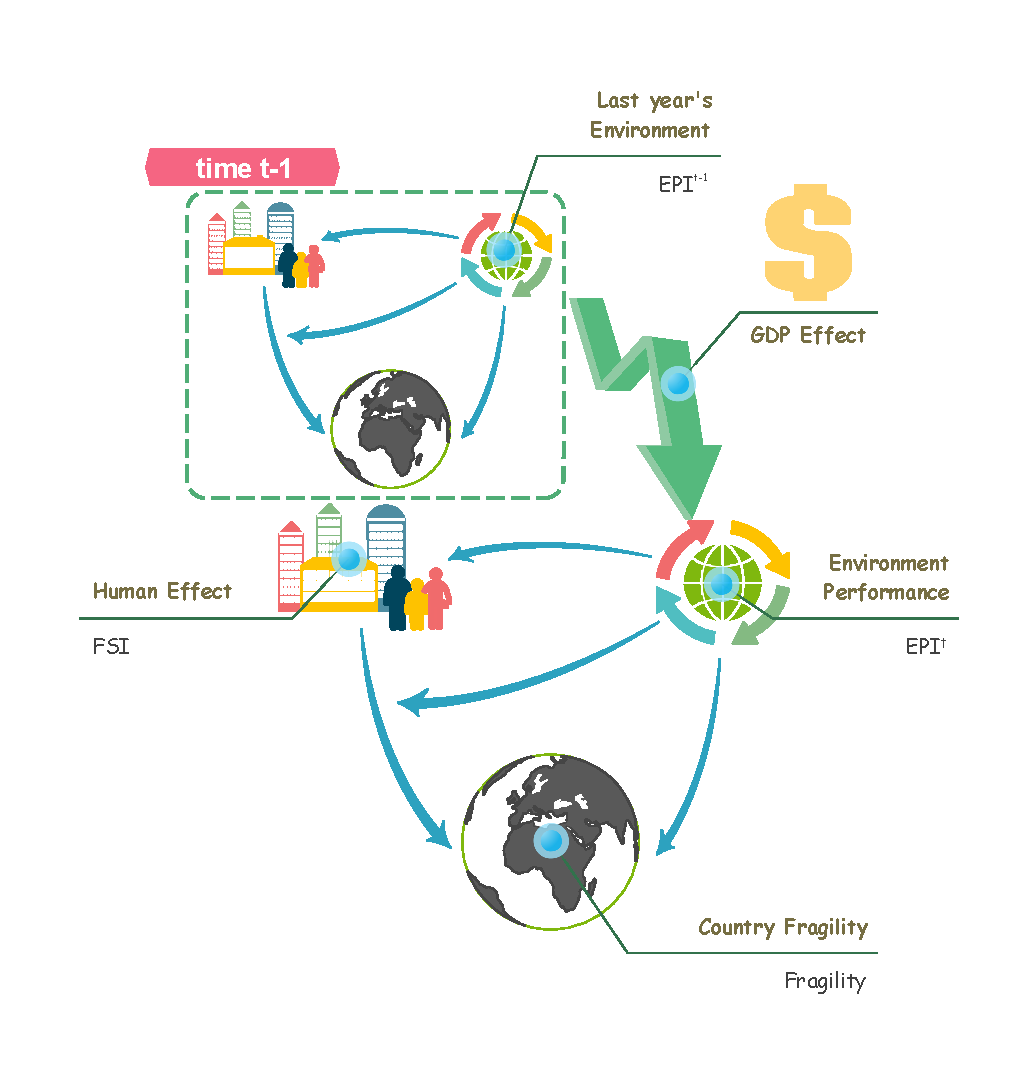
\includegraphics[width=.5\linewidth]{figs/model.eps} 
   \caption{Hypothesis Model Illustration}
   \label{fig:model:model}
\end{figure}

\begin{figure}[t]
   \centering
   \subfigure[Moderator variable model]{
       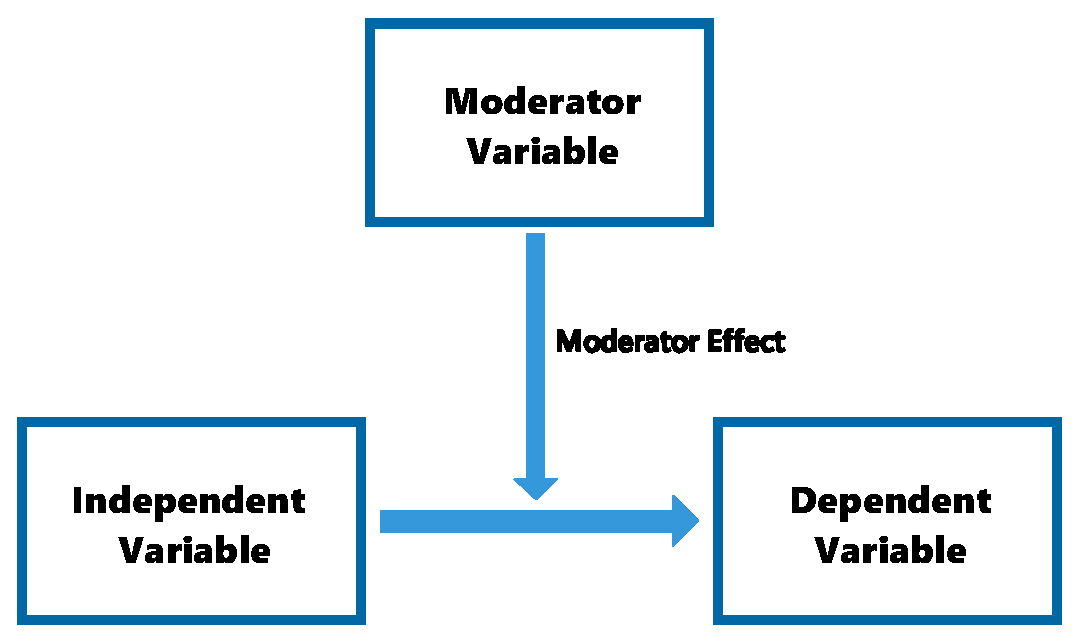
\includegraphics[width=.4\linewidth]{figs/model_moderator.eps}
       \label{fig:model:indirect:moderator}
   } 
   \subfigure[Mediator variable model]{
       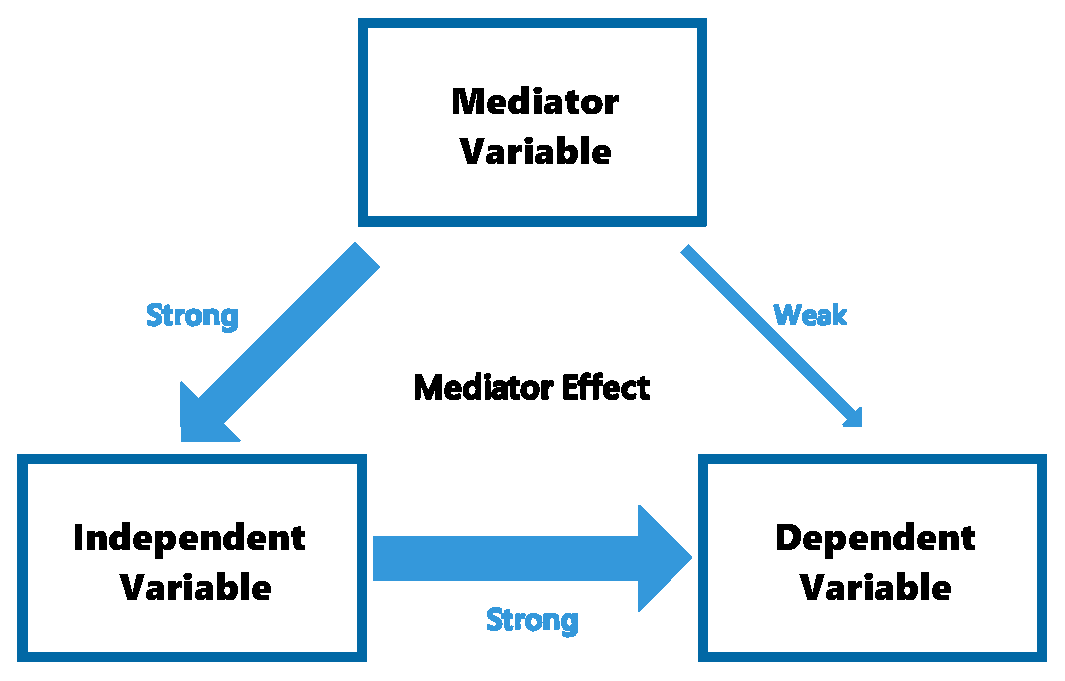
\includegraphics[width=.4\linewidth]{figs/model_mediator.eps}
       \label{fig:model:indirect:mediator}
   }
   %\label{fig:model:indirect}
   \caption{Hypothesis models for indirect effect of environmental factors. $\EFF$ represents environmental factors, $\HFF$ represents human factors, and $\FFF$ represents state fragility. The fragility is jointly determined by $\EFF$ and $\HFF$, by two hypothesis approach.}
\end{figure}
\label{sec:model}
In this part we propose theoretical framework for our analysis of the impact of climate change on \emph{state fragility}.
\subsection{Assumptions and Model Framework}
Our hypothesis framework is illustrated in Figure~\ref{fig:model:model}.
We propose two natural assumptions, based on which we derive the basic framework of our model. 
\begin{enumerate}
   \item The \emph{state fragility}, a concept to estimate the sustainability of states, is dependent on and only on \emph{human factors} and \emph{environmental factors.} \label{model:assump:1}
   \item The environmental factors and human factors interact with each other. \label{model:assump:2}
\end{enumerate}
The assumptions are natural. Assumption~\ref{model:assump:1} requires to quantify the fragility which considers both human factors and environmental factors. We propose a novel framework to quantify fragility by incorporating the human and environmental factors into a probabilistic framework.

Assumption~\ref{model:assump:2} requires a more sophisticated analysis of the two factors, including their respective and joint effects on the fragility, and the interaction between them. We are especially interested in the effects of environmental factors, which include \emph{direct} effect, which is the influence on fragility directly imposed by environmental factors; and \emph{indirect} effect, which is the influence on fragility imposed by envirionmental factors indirectly through human factors. Two hypothesis model to explain the indirect effect is visualized in Figure~\ref{fig:model:indirect:moderator} and~\ref{fig:model:indirect:mediator}.

The direct effect of environmental factors is measured by the effect of environmental factors on fragility score, with an unbiased estimation of the effect obtained by propensity score matching~\cite{caliendo2008some,dehejia2002propensity,hirano2004propensity}. The indirect effect of environmental factors can be explained by two hypothesis models: the \emph{moderator variable} model, as shown in Figure~\ref{fig:model:indirect:moderator}; and the \emph{mediator variable} model, as shown in Figure~\ref{fig:model:indirect:mediator}. We verify these two hypothesis.

In the following of this section, we are dedicated to enrich our model by developing several key ingredients: 
\begin{enumerate}
   \item A novel fragility score measure incorporating both environmental and human factors;
   \item The interaction pattern between human factors, envirionmental factors, and the fragility;
   \item The temporal model of a state's environmental status.
\end{enumerate}

The basic framework is sufficient to cover most of the requirements of the tasks.

\subsection{Representing the Two Factors}
\label{sec:model:rep}
\begin{table}[htbp]
   \centering
   \begin{tabular}{|c|c|} \hline 
      Notation & Description \\ \hline
      $\HFF $  & random variable of human factors \\ \hline
      $\EFF $ & random variable of environmental factors \\ \hline
      $ \FFF $ & binary random variable of fragility \\ \hline
      $\FFS $ & fragility score \\ \hline
   \end{tabular}
   \caption{Notations}
   \label{tab:model:notations}
\end{table}

\hide{
\begin{figure}[t]
    \centering
    \subfigure[FSI]{
        \includegraphics[width=.45\linewidth]{figs/fsi.eps}
        \label{fig:model:indexes:fsi}
    }
    \subfigure[EPI]{
        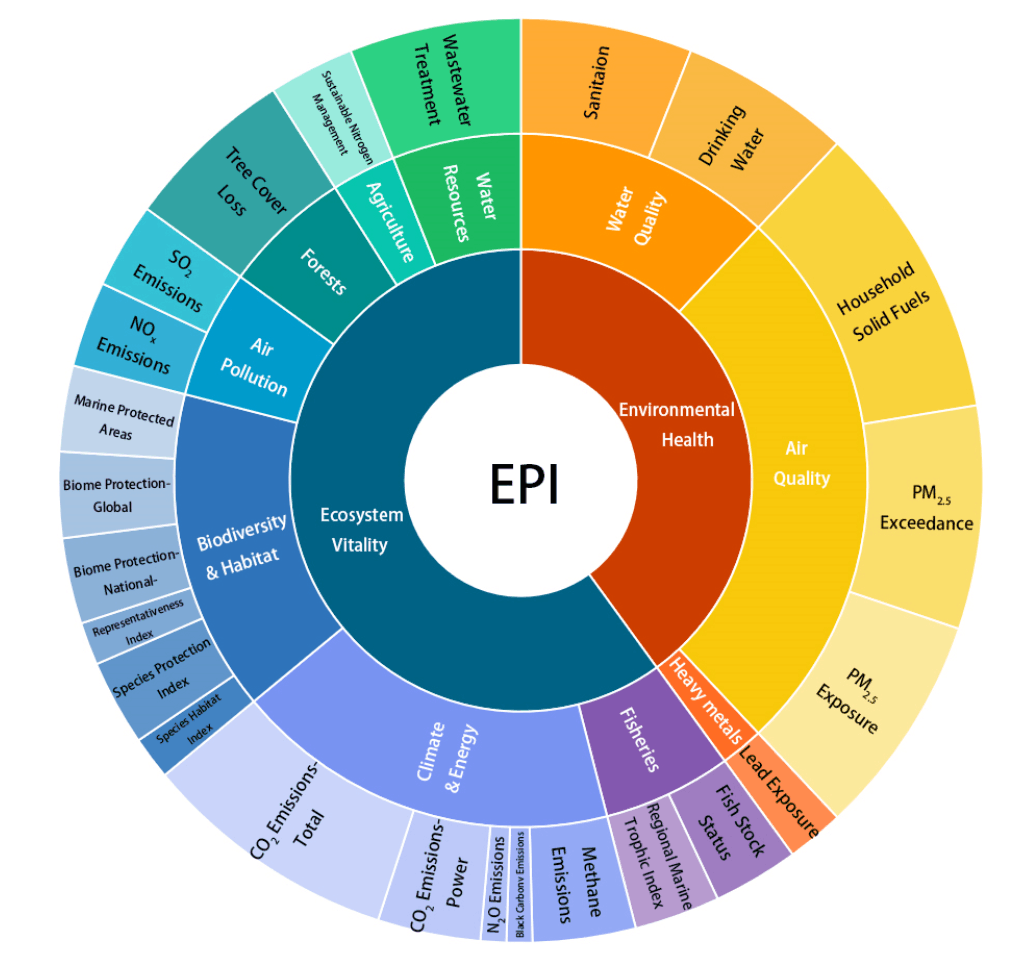
\includegraphics[width=.45\linewidth]{figs/epi.eps}
        \label{fig:model:indexes:epi}
    }
    \caption{The two fragiliy indexes.}
    \label{fig:model:indexes}
\end{figure}
}

\begin{figure}[htbp]
   \centering
   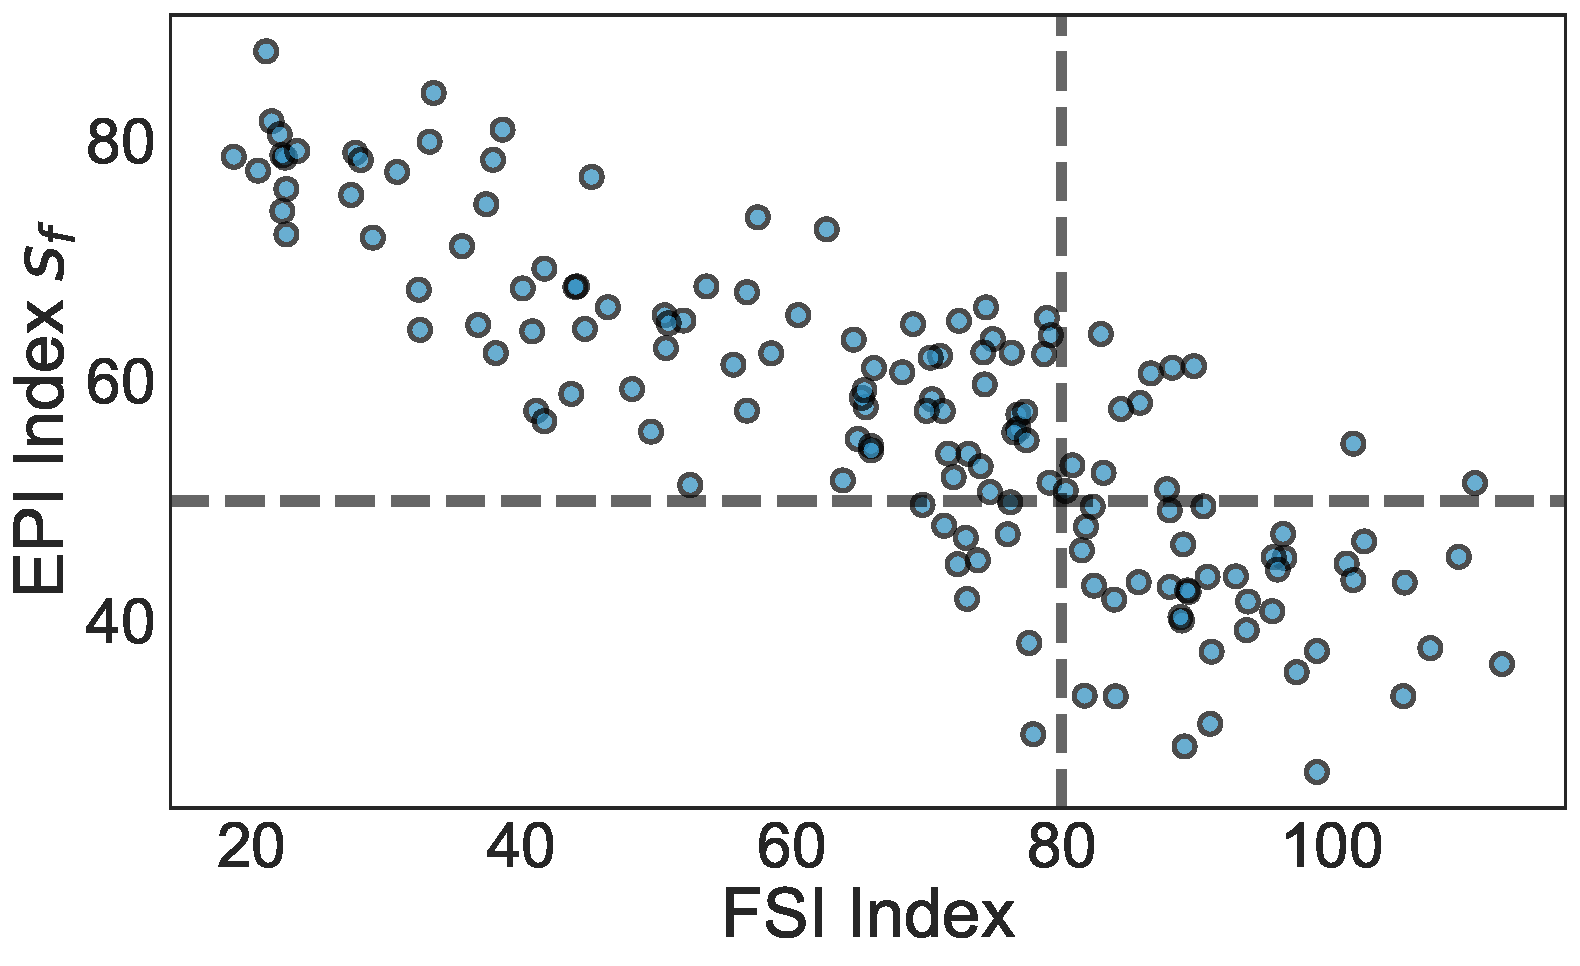
\includegraphics[width=.4\linewidth]{figs/fsiepi}
   \caption{EPI and FSI Indexes}
   \label{fig:model:epifsi}
\end{figure}

Basic notations are listed in Table~\ref{tab:model:notations}.
The variables in the table are theoretical. In order to reflect these variables numerically from empirical data, we introduce two widely recognized indexes:

\vpara{Environmental Performance Index (EPI).} It is an index to evaluate a state's environmental performance developed by Yale University~\cite{EPI_index}. It is composed of indicators in ecosystem vitality and environmental health. The higher the index, the better the environment, 

\vpara{Fragile States Index (FSI).} It is an index to measure a country's vulnerability to conflict developed by Fund for Peace and Foreign Policy by accounting for 12 social, economical, and political indicators.~\cite{FSI_index} Higher index indicates more vulnerability.

FSI index uses indicators relevant to human activity, and is therefore used as empirical data for $\HFF$. 
EPI index measures environmental fragility, and is therefore used as empirical data for $\EFF$.

Sometimes, we use binarized values of EPI and FSI indexes to denote the status of a state. The threshold and the relation between EPI and FSI are visualized in Figure~\ref{fig:model:epifsi}. 

\subsection{Probabilistic Fragility Measure}
\label{sec:model:frag}
In this part, we derive a novel fragile score, $\FFS$, which incorporates both environmental and human factors. The score $\FFS$ is based on probabilistic intuitions, and is therefore called the \emph{probabilistic fragility score}, or the fragility score for convenience.

Without loss of generality, we refer to regions, sovereign states, and other concerned geographical entities as states.

We assume that a state either fragile or stable, described by a binary random variable $\FFF$, where $\FFF=1$ if the considered state fragile, and $\FFF=0$ if it is stable. $\HFF$ and $\EFF$ are random variables describing the human and environmental factors of the state. For convenience, we further assume that $\EFF$ is binary, i.e. $\EFF=1$ when the state's environment is sustainable, and $\EFF=0$ when it is not. 

Consider the probability of a state being fragile, given its human and environmental factors:
\begin{equation}
    \prob{(\FFF=1|\EFF=e, \HFF)} \ \ (e=0,1)
\label{eqn:model:frag_prob}
\end{equation}

The probability given in~\ref{eqn:model:frag_prob} quantifies the extent of fragility of the state, given certain environmental and human factors. It is higher when the state is more vulnerable. However, the conditional distribution is hard to estimate. We then factorize it into a more easily calculated form: 
\begin{equation}
    \prob(\FFF=1|\EFF=e,\HFF)= \frac{\prob(\EFF=e, \FFF=1 | \HFF)}{\prob(\EFF=e | \HFF)} = \frac{\prob(\mathbf{Z}=1|\HFF)}{\prob(\EFF=e|\HFF)}\ \ (e = 0,1)
    \label{eqn:model:frag_prob_fact}
\end{equation}
In which we defined a new random variable $\mathbf{Z}=1$ if $\EFF=e,\FFF=1$ and $\mathbf{Z}=0$ otherwise.
Eqn.~\ref{eqn:model:frag_prob_fact} allows us to only estimate the conditional probability of two binary random variables given human factors $\HFF$.

For convenience of calculation, we assume linear relationships: 
\begin{eqnarray}
   \log\frac{\prob(\mathbf{Z}=1|\HFF)}{\prob(\mathbf{Z}=0|\HFF)} & = & \mathbf{W}_1\HFF + \mathbf{e}_1 \nonumber \\
   \log\frac{\prob(\mathbf{\EFF}=e|\HFF)}{\prob(\mathbf{\EFF}=1-e|\HFF)} & = & \mathbf{W}_2\HFF + \mathbf{e}_2 
   \label{eqn:model:logistic_form}
\end{eqnarray}

Where $\mathbf{W}_i$ are parameters, $\mathbf{e}_i$ are Gaussian errors, $i=1,2$.

Using the linear assumption and the logistic form in Eqn~\ref{eqn:model:logistic_form}, we obtain the estimate of the probabilities respectively:

\begin{eqnarray}
   \hat{p}_z & = & \frac{\exp(\mathbf{W}_1\HFF)}{1+\exp(\mathbf{W}_1\HFF)} \nonumber \\
   \hat{p}_e & = & \frac{\exp(\mathbf{W}_2\HFF)}{1+\exp(\mathbf{W}_2\HFF)}
   \label{eqn:model:prob_estimate}
\end{eqnarray}

In order to make the estimated probability distribution resemble the true distribution, we estimate parameters $\mathbf{W}_1, \mathbf{W}_2$ by minimizing the cross entropy loss, which is equivalent to minimizing the KL divergence~\cite{deeplearning} between the estimated distribution and the empirical distribution. Specifics of optimization are omitted; interested readers may see \cite{deeplearning}.

Finally, probabilities in Eqn.~\ref{eqn:model:frag_prob_fact} is replaced by the estimates given in Eqn.~\ref{eqn:model:prob_estimate}, yielding the \emph{probabilistic fragility score}:
\begin{equation}
  \label{eqn:model:frag_score}  
  \FFS = \frac{\hat{p}_z}{\hat{p}_e}
\end{equation}

\paragraph{Notes on the fragility score.} The fragility score, $\FFS$, is derived based on probabilistic intuitions and linear assumptions. Higher $\FFS$ indicates higher risks of being fragile. However, the score $\FFS$ can be larger than one, and is, therefore, not in form of probability. However, it does not hurt its applicability: if the estimated $\hat{p}_z$ is larger than $\hat{p}_e$, we have even more reasons to believe that the considered state is fragile. 

\subsection{Modeling the Interaction between Variables}
We then begin to model the relationship between the three variables: environmental factors $\EFF$, human factors $\HFF$, and the fragility score $\FFS$. 

\subsubsection{Direct Effect of Environmental Factors} In order to measure the effect of environmental factors on fragility score, a naive approach would be to sample states of both sustainable environment and unsustainable environment, and compare their average fragility score. Formally, write $s^0_f$ as the average fragility score of the sustainable group, and $s^1_f$ as the average fragility score of the unsustainable group. One then compares the difference $s^*_f=s^0_f - s^1_f$.

The above approach gives, however, biased estimation, because the apparent difference between these two groups may be depend on human factors that affected whether or not a state's environment is sustainable, instead of the environmental status per se. For example, the approach might compare scores of the states that are environmentally unsustainable and in political turmoil, with the scores of the states that are environmentally sustainably and politically stable. The difference of political status results in unbiased estimate of the effect of environmental factors.

To control for the differences of human factors between the sustainable group and the unsustainable group, we use the propensity score matching, a statistical technique that attempts to estimate unbiasly the effect of a variable, in this case, the environmental status.

Formally, the propensity score of a certain state is defined as the conditional probability of the environmental status given its human factors,
\begin{equation}
   p=\prob(\EFF=1|\HFF)
   \label{eqn:model:propensity}
\end{equation}
%\reminder{environmental status? environmental factors? they are probably different.}
In order to estimate the probability, we adopt similar procedures used in Section~\ref{sec:model:frag}, using the score of logistic regression, $\hat{p}$, of human factors $\HFF$ against environmental status $\EFF$. Then we match each of the unsustainable states to one sustainable state on propensity score, by using \emph{Nearest Neighbor Matching}: each unsustainable state is matched to the sustainable state whose propensity score is the closest. As such, a new data set in which the sustainable group and the unsustainable group and their propensity scores are balanced, is obtained. 

Based on the newly obtained data set, we calculate the adjusted score difference:
\begin{equation}
   \hat{s}^*_f=\hat{s}^0_f - \hat{s}^1_f.
   \label{eqn:model:score_diff_adj}
\end{equation}

Where $\hat{s}^0_f$, $\hat{s}^1_f$ are average scores of the sustainable and unsustainable group, drawn from the data set obtained by PSM.

\subsubsection{Indirect Effect of Environmental Factors}
\label{sec:model:indirect}
In order to measure the indirect effect of environmental factors $\EFF$, we propose two candidate models: the moderator variable model, and the mediator variable model.

%\reminder{is the difference clearly explained?}
The moderator variable model assumes that the environmental factors influence the fragility score, and the relationship is calibrated by the effect of human factors. 
In this case, the human factors $\HFF$ are called \emph{the moderator variable}, as illustrated in Figure~\ref{fig:model:indirect:moderator}.~\cite{baron1986moderator}

The mediator variable model assumes that the environmental factors and human factors jointly influence the fragility score.
Furthermore, the environmental factors influence the fragility score both directly, and indirectly through the human factors. The illustration of this model is as in Figure~\ref{fig:model:indirect:mediator}.~\cite{aiken1991multiple}

\vpara{Moderator variable model.}
The model is written as 
\begin{equation}
    \FFS = \mathbf{W}_1\HFF + W_2\EFF + \sum_{i=1}^p \beta_i h_i \EFF 
    \label{eqn:model:moderator_model}
\end{equation}
where $\HFF=\left[ h_1,\ldots,h_p \right]'$, and $h_i$ is the $i$th component of $\HFF$, indicating a specific factor. $\mathbf{W}$ and $\beta_i$ are parameters.

The term, $\sum_{i=1}^p\beta_i h_i$, represents the effect of each human factor on the relation between the environmental factor and the fragility score, since by taking partial derivative, we observe that 
\begin{equation*}
    \frac{\partial s_f}{\partial \EFF} = W_2 + \sum_{i=1}^p \beta_i h_i
\end{equation*}
The derivative indicates that the effect of environmental factor $\EFF$ comes from both itself, described by $W_2$, and each human factor $h_i$, described by $\beta_i$. If the factor $h_i$ has no effect on the relation, then $\beta_i$ should be close to zero. Consider, therefore, the following statistical test:
\begin{equation}
    H_0: \beta_1=\beta_2=\ldots=\beta_p
    \label{eqn:model:moderator:testall}
\end{equation}
The rejection of $H_0$ shows that the moderator effect of $\HFF$ is significant. 
Furthermore, we wish to specifically investigate the effect of each factor. Hence in the following test,
\begin{equation}
   H_0:\beta_i=0 
   \label{eqn:model:moderator:testi}
\end{equation}
if $H_0$ is rejected, we are confidence to say that the moderator effect of $h_i$ is statistically significant.

If the moderator effect is indeed significant, then the extent of the effect of $\HFF$ is then quantified by $\mathbf{\beta} = \left[\beta_1,\ldots,\beta_p\right]'$ and respective components.

\vpara{Mediator variable model.} 

We first declare the following values:
\begin{itemize}
   \item $b_1$: the coefficient of the linear regression model, in which $\EFF$ predicts $\FFS$.
   \item $b_2$: the coefficient of the linear regression model, in which $\HFF$ predicts $\FFS$.
   \item $b_3$: the coefficient of $\EFF$ in the linear regression model in which $\EFF$ and $\HFF$ jointly predicts $\FFS$.
   \item $b_4$: the coefficient of $\HFF$ in the linear regression model in which $\EFF$ and $\HFF$ jointly predicts $\FFS$.
\end{itemize}

First, we need to verify by statistical tests that $b_1$ and $b_2$ are significantly nonzero.

If $\HFF$ indeed acts as a mediator variable, by model assumption, $b_4$ is significantly nonzero. Furthermore, since $\EFF$ indirectly influences $\FFS$ through $\HFF$, the explaining power of $\EFF$ alone should be reduced once $\HFF$ is introduced. In this case, $b_3 < b_1$.

If all the above four conditions hold significantly, we are confident to say that human factors act as mediator variables, through which the environmental factors influence the fragility score.